\chapter{How to Write a Bestselling Novel}

This lecture begins by tempting us in the wrong direction. We are shown the den, the secret door, the shelves, the place where the books are made, and then the temptation is immediately withdrawn: one can write in an airport lounge, on a plane, in a car. The lesson is not the room. The lesson is the process. From there the interview unfolds as a sequence of linked problems: how information is arranged, how comments become diagnoses, why revision is treated as recomposition, how long that recomposition takes, and what one does when a long manuscript suddenly seems unreadable.

\section{The Room, and the Swift Turn to Method}

The opening is useful precisely because it is misleading for a moment. We begin with place, but the lecturer refuses to let place carry explanatory weight. The den is pleasant. It may even be the best place. But writing, we are told, can happen elsewhere. This clears the ground for the real subject: not ambience, but method.

That first turn matters. A weaker lecture would remain at the level of writerly atmosphere. This one does not. It treats the room as entry and the process as substance. We are therefore prepared, almost immediately, for the real pivot: the three-screen setup and the mechanics of how a novel moves from draft to draft.

\subsection{Question \& Answer}

\paragraph{Question.} Does a writer need the ideal room, or only a working process?

\paragraph{Answer.} The lecture's answer is that a good room is helpful but not decisive. What matters is a repeatable process. The room may support the work; it does not explain the work.

\section{Three Screens and the Flow of Revision}

Once the room has been demoted, the interview becomes technical. We are shown a process rather than a mood. One screen holds the first draft. Another holds comments from readers who have seen that draft. In the middle sits the second draft in progress. The arrangement is simple enough to write as a map:
\begin{equation}
\text{first draft} \to \text{reader comments} \to \text{second draft}.
\end{equation}
This is the first real mathematical spine of the lecture. It says that writing is not merely production, followed by vague reflection. It is a controlled flow of material through response into reconstruction.

We can sharpen the same point in a second way:
\begin{equation}
\text{reader response} \to \text{diagnosis} \to \text{revision priority}.
\end{equation}
A comment is not important merely because it was uttered. It becomes important when it reveals what the manuscript is actually doing to a reader.

\begin{definition}
A \emph{revision priority} is a comment or diagnosis that rises to the top because it identifies a structural weakness rather than a merely local preference.
\end{definition}

Since no validated visual evidence of the monitor layout survives, we record the arrangement schematically rather than pictorially:

\begin{figure}[h]
\centering
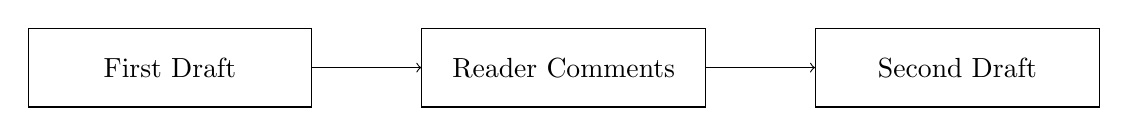
\begin{tikzpicture}
\node[draw, rectangle, minimum width=3.6cm, minimum height=1cm] (A) at (0,0) {First Draft};
\node[draw, rectangle, minimum width=3.6cm, minimum height=1cm] (B) at (5,0) {Reader Comments};
\node[draw, rectangle, minimum width=3.6cm, minimum height=1cm] (C) at (10,0) {Second Draft};
\draw[->] (A) -- (B);
\draw[->] (B) -- (C);
\end{tikzpicture}
\end{figure}

This reconstruction is deliberately minimal. The lecture is not giving us a fetish of equipment. It is showing a workflow: the draft is exposed, the responses are collected, and the next draft is written under the pressure of what has been learned.

\subsection{Question \& Answer}

\paragraph{Question.} What information belongs in front of the writer while revising?

\paragraph{Answer.} The lecture's answer is exact: the current draft, the responses it has produced, and the space in which the next draft is being composed. Revision becomes clearer when these are held in explicit relation.

\section{From Comment to Diagnosis: Pace as a Measurable Craft Problem}

The lecture then shows the system in operation. One reader says that they were not drawn in as quickly and did not read the new book as fast as the last two. Follett does not take this as injury. He takes it as data. The inference is immediate:
\begin{equation}
\text{not drawn in quickly} \Rightarrow \text{opening chapter may be ponderous}.
\end{equation}
This is a model act of craft reasoning. The surface comment is translated into a structural problem.

That problem is then compared with a pacing heuristic that Follett states explicitly:
\begin{equation}
\text{plot twist interval} \approx 3\text{--}4 \ \text{pages}.
\end{equation}
The rule is not presented as a universal theorem of fiction. It is presented as a working measure of narrative pull. If the opening is not turning often enough, then the reader's slower engagement is no mystery.

\paragraph{Worked example.} The reasoning may be written in steps:
\begin{enumerate}
\item A reader reports being drawn in too slowly.
\item The writer refuses to hear this as a personal slight.
\item The report is translated into a structural hypothesis: the opening may be ponderous.
\item That hypothesis is tested against a pacing heuristic.
\item The comment therefore rises to high revision priority.
\end{enumerate}

The interviewer then asks the necessary question: would an established writer simply dismiss such a comment? The answer gives us another compact relation:
\begin{equation}
\text{feedback} \neq \text{insult}, \qquad
\text{feedback} \Rightarrow \text{what can I learn?}
\end{equation}
That equation matters. Without it, the whole three-screen system would collapse into vanity. With it, response becomes instrument rather than affront.

\subsection{Question \& Answer}

\paragraph{Question.} How does a comment become a structural diagnosis?

\paragraph{Answer.} By being converted from reaction into craft language. ``I was not drawn in quickly'' becomes not a taste judgment but a statement about pace, and then a target for revision.

\section{The Second Draft as Recomposition}

The lecture's strongest claim comes next. Follett says that when he moves to the second draft, he does not take the first draft and merely alter it. He does not edit in the ordinary sense. He types the book again. The distinction is strong enough to deserve formal statement:
\begin{equation}
\text{second draft} \neq \text{annotated first draft}, \qquad
\text{second draft} = \text{book rewritten from scratch}.
\end{equation}
This is more radical than routine advice about revision. The second draft is not a corrected version of the first object. It is a new construction produced under better information.

That is why the process screen in the center matters so much. The center is not a site of repair only. It is the place where the book is made again. Comments and earlier pages are guides, but they are not the thing being cosmetically improved.

\subsection{Question \& Answer}

\paragraph{Question.} Why rewrite the whole book instead of simply editing the first draft?

\paragraph{Answer.} Because on this view the first draft is not yet the proper object of polish. It is material, evidence, and occasion for diagnosis. The second draft is where the book is rebuilt under higher standards and clearer understanding.

\begin{remark}
The lecture presents this as Follett's method and conviction. It should be preserved as a strong working standard inside the interview, not inflated into a universal law of all fiction writing.
\end{remark}

\section{The Arithmetic of a Long Novel}

Once the method is stated, the interviewer raises the natural objection: this must take longer. Follett's answer is not evasive. It is arithmetic:
\begin{equation}
\text{planning} = 1\ \text{year}, \qquad
\text{first draft} = 1\ \text{year}, \qquad
\text{second draft} = 1\ \text{year}.
\end{equation}
The implied project horizon is therefore
\begin{equation}
T_{\text{book}} = T_{\text{plan}} + T_{\text{draft1}} + T_{\text{draft2}}.
\end{equation}
This is one of the lecture's cleanest contributions. It turns a vague sense that novels take time into a decomposed temporal structure.

The next challenge follows naturally. If the second draft costs so much, is it really essential? Follett's answer is yes. Publishers may sometimes want to publish the first draft, but, in his view, that reflects a lower standard. His own conclusion can be written:
\begin{equation}
\text{rewrite from scratch} \Rightarrow \text{better product}.
\end{equation}
Again, the statement is local to the lecture, not universal metaphysics. But it is central to the interview's logic. The time-cost is justified because the resulting book is better.

A second transcript-based schematic is useful here:

\begin{figure}[h]
\centering
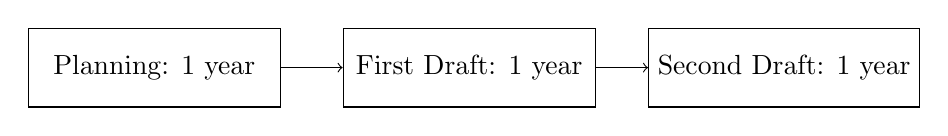
\begin{tikzpicture}
\node[draw, rectangle, minimum width=3.2cm, minimum height=1cm] (P) at (0,0) {Planning: 1 year};
\node[draw, rectangle, minimum width=3.2cm, minimum height=1cm] (F) at (4,0) {First Draft: 1 year};
\node[draw, rectangle, minimum width=3.2cm, minimum height=1cm] (S) at (8,0) {Second Draft: 1 year};
\draw[->] (P) -- (F);
\draw[->] (F) -- (S);
\end{tikzpicture}
\end{figure}

The point of this figure is not decoration. It makes plain that the lecture treats quality as distributed across stages rather than concentrated in a single act of inspiration.

\section{Severe Doubt in the Middle, and the Rule for Continuing}

The lecture then pivots inward. The interviewer asks about angst, writer's block, and crisis. Follett refuses the grand language of the tortured soul, but he does not deny difficulty. Instead he names a recurring moment in every book: one is deep into the manuscript, several hundred pages have been written, and suddenly the thought comes, why would anybody want to read this?

That moment may be represented as
\begin{equation}
\text{hundreds of pages written} \Rightarrow \text{severe doubt}.
\end{equation}
The force of the lecture lies in what happens next. The answer is not revelation, self-expression, or panic. It is operational:
\begin{align}
\text{doubt} &\Rightarrow \text{press on} \Rightarrow \text{rewrite later if needed},\\
\text{if draft is not good enough} &\Rightarrow \text{rewrite} \Rightarrow \text{improvement}.
\end{align}
This is perhaps the lecture's most practical theorem. A psychological collapse is resolved by procedural trust. One does not stop and let the feeling rule. One continues, protected by the knowledge that revision exists.

\subsection{Question \& Answer}

\paragraph{Question.} What should we do when a book suddenly seems unreadable to its own author?

\paragraph{Answer.} The lecture's answer is deliberately unspectacular: continue. Put the thought aside, finish the work in front of you, and trust revision to pass judgment later. The feeling of unreadability is not granted final authority.

\section{Standards, Absorption, and Love of the Work}

The lecture could have ended on doubt and endurance, but it does not. It chooses a stronger resolution. Follett recalls being told that his problem as a writer was that he was not a tortured soul. He loves the process. He is absorbed by it. That closing relation is not trivial:
\begin{equation}
\text{absorption in work} \Rightarrow \text{endurance of process}.
\end{equation}
This clarifies everything that came before. The three screens, the full rewrite, the three-year structure, the refusal to stop in the middle of doubt: all of these can be sustained because the work is not merely tolerated. It is adored.

This also brings the lecture back to its hidden opening contrast. The room was never the source of the magic. The method was. And the method remains livable because it is animated by attachment rather than by grim self-punishment.

\section{Summary}

The lecture advances by turning one form of romance after another into method. It begins with the den, then refuses to treat the room as the secret. It moves to the three-screen workflow, where drafting, feedback, and rewriting are organized into a visible process. A single reader comment is translated into a diagnosis of pace and then measured against the heuristic of a twist every three to four pages. Revision is then redefined: the second draft is not an annotated first draft, but a new book rewritten from scratch. The arithmetic of this standard becomes explicit in the one-year decomposition of planning, first draft, and second draft. Finally, the lecture confronts the severe doubt that appears after several hundred pages and answers it with a rule of continuation backed by trust in revision. The closing note matters as much as the method itself: rigor is sustainable because the work is loved.